\chapter{Introduction}
\label{chap:Introduction}
Software bugs are an inherent part of programming, often leading to unexpected behaviour and system failures. Debugging these errors is a \textit{time-consuming process} taking between 20-60\% of active work time \cite{DebugTimeSelfReport}, with programmers spending a \textit{highly skewed} proportion of their time identifying and resolving a small proportion of \textit{difficult} bugs \cite{DebugSkew}.

Type systems aim to alleviate some of this burden by classifying expressions and operations that are allowed to work on them. This may be done \textit{statically} at compile time or \textit{dynamically} during runtime. The expressions not conforming to the type system manifest themselves as \textit{type errors}.

In static typing, blame for type errors are typically localised to a \textit{single} location in the code. However, this localisation may be misleading, as the actual cause of the error might be rooted in a broader context, for example in OCaml 65\% of type errors related to \textit{multiple} locations \cite{StudentTypeErrorFixes}. This is a particularly prevalent issue in \textit{type inferred} languages.

In dynamic typing, type errors are often missed as they only appear during runtime with specific inputs.
Additionally, they don't generally specify any source code context which caused them. Instead, a dynamic type error is accompanied by an \textit{evaluation trace}, which can be \textit{more intuitive} \cite{TraceVisualisation} by demonstrating concretely why values are \textit{not} consistent with their expected type as required by a \textit{runtime cast}.

This project seeks to improve user understanding of type errors by localising static type errors \textit{more completely}, and \textit{combining} the benefits of static and dynamic type errors.

I consider three research problems and implement three features to solve them in the Hazel language \cite{Hazel}:\footnote{The answers may differ greatly for other languages. Hazel provides a good balance between complexity and usefulness.}
\begin{enumerate}
\item Can we statically highlight code which explains \textit{static type errors} more \textit{completely}, including all code that \textit{contributes} to the error? 

This would alleviate the issue of static errors being \textit{incorrectly localised}, and help give a \textit{greater context} to static type errors.

\textbf{Solution:} I devise a \textit{novel} method of \textbf{type slicing} including formal mathematical foundations built upon the formal \textit{Hazel calculus} \cite{HazelLivePaper}. Additionally, it generalises to highlight all code relevant to typing \textit{any} expressions (not just erroneous expressions).

\item Can we dynamically highlight source code which contributes to a \textit{dynamic type error}?

This would provide missing source code context to understand how types involved in a dynamic type error originate from the source code.

\textbf{Solution:} I devise a \textit{novel} method of \textbf{cast slicing}, also with formal mathematical foundations. Additionally, it generalises to highlight source code relevant to requiring any specific \textit{runtime casts}.

\item Can we provide dynamic \textit{evaluation traces} to explain \textit{static type errors}?

This would provide an \textit{intuitive} concrete explanation for static type errors.

\textbf{Solution:} I implement a \textbf{type error witness search procedure}, which discovers inputs (witnesses) to expressions which cause a \textit{dynamic type error}. This is based on research by Seidel et al. \cite{SearchProc} which devised a similar procedure for a subset of OCaml.
\end{enumerate}

Hazel \cite{Hazel} is a functional locally inferred and gradually typed research language allowing the writing of \textit{incomplete programs} under active development at the University of Michigan. Being gradually typed, allowing both static and dynamic code to coexist, this project successfully demonstrates the utility of these three features in improving understanding of \textit{both} static and dynamic errors. Both, to a \textit{greater extent} than in any existing languages, with the explanations being \textit{useful} in debugging type errors, and expected to aid in building understanding of bidirectional type systems.

\paragraph{Example:} \Cref{fig:ErrorExample} shows an attempt at writing a int list concatenation function. But list cons (\code{::}) is used instead of list concatenation (\code{@}). Type slicing will automatically highlight the code that caused \code{x} to synthesise the \code{[Int]} type and the code that enforces the requirement that \code{x} is an \code{Int}. If the error is still not clear, the search procedure can be used to generate inputs which evaluate to cast errors, for example \code{concat([[], []])}, giving a concrete evaluation trace to an error. Finally, cast slicing will allow the cast errors to be selected, highlighting source code that enforced the cast, in general being a more concise slice than statically found by type slicing and which is also being. The results of this example among others are explored in the evaluation (\cref{sec:EvalExamples}).

\begin{figure}[h]
\centering
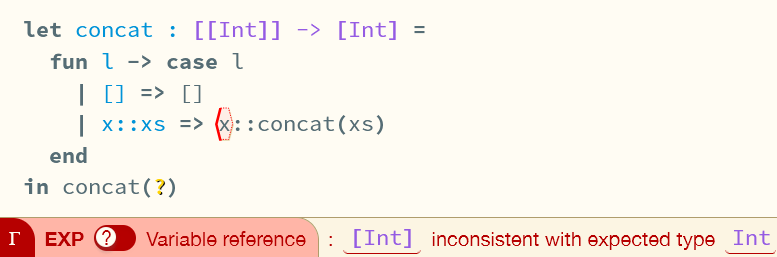
\includegraphics[width=0.7\textwidth]{Media/Figures/concat_error}
\caption{A Static Type Error}
\label{fig:ErrorExample}
\end{figure}

\section{Related Work}
\label{sec:RelatedWork}
There has been extensive research into the field of programming languages and debugging, attempting to understand \textit{what} is needed \cite{DebugNeeds}, \textit{how} developers fix bugs \cite{HowFixBugs}, and a plethora of compiler improvements and tools. This project builds upon this body of research in new ways focusing on the Hazel language, which is itself a research project being taken in various directions but of particular note as a \textit{teaching language} \cite{HazelTutor} for students, where this features can additionally help with teaching understanding of bidirectional type systems. 

To my knowledge the ideas of \textit{type slicing} and \textit{cast slicing} are novel. However, they do output \textit{program slices} which were originally explored by Weiser \cite{ProgSlice}, though my definition of program slices matches more with functional program slices \cite{FunctionalProgExplain}.  The properties I explore are more similar to \textit{dynamic program slicing} \cite{DynProgSlice} but with type characteristics rather than evaluation characteristics, in a sense similar \textit{type error slicing}\cite{ErrSlice, HaackErrSlice}.

The \textit{type witness search procedure} is	 based upon Seidel et al. \cite{SearchProc}, though there are significant differences in workings due to my use of Hazel and various extensions as compared to the subset of OCaml used by Seidel et al.

\section{Dissertation Outline}
\label{sec:Outline}
\Cref{chap:Preparation} introduces the \textit{type theories} (\cref{sec:TypeSystems}) underpinning the \textit{Hazel core calculus} (\cref{sec:CoreHazel}), followed by basic background on the \textit{Hazel implementation} (\cref{sec:HazelImplementation}), and methods of non-deterministic programming (\cref{sec:Nondeterminism}).

\Cref{sec:TypeSlicingTheory} and \cref{sec:CastSlicingTheory} conceive and formalise the ideas of \textit{type slices} and \textit{cast slices} applied to the Hazel core calculus. 
 
 An implementation (\cref{sec:TypeSlicingImplementation}-\ref{sec:CastSlicingImplementation}) of the slicing theories was created covering \textit{most}\footnote{Except for type substitution.} of the Hazel language, including a user interface. 
 
 A \textit{type witness search procedure} was successfully implemented (\cref{sec:SearchProcedure}). This involved created a non-deterministic evaluation method (\cref{sec:IndetEval}) abstracting search order and search logic.

The slicing features and search procedure met all goals\footnote{Including those on the project proposal, this evaluation is more extensive.} (\cref{sec:EvaluationGoals}), showing \textit{effectiveness} (\cref{sec:EffectivenessAnalysis}) and being reasonably \textit{performant} (\cref{sec:PerformanceAnalysis}) over a corpus of \textit{well-typed} and \textit{ill-typed} Hazel programs respectively (\cref{sec:CorpusCollection}). Further, the features weaknesses were evaluation, with considered improvements implemented or devised (\cref{sec:CriticalAnalysis}). Additionally, a holistic evaluation was performed (\cref{sec:HolisticEvaluation}), considering the use of all the features, in combination with Hazel's existing error highlighting, for debugging both static and dynamic type errors.

Finally, further directions and improvements have been presented in \cref{chap:Conclusions}.